\subsection{Elektrische Konstruktion}
Unser CanSat besteht aus mehreren Sensoren und einem zentralen Verarbeitungssystem sowie einem Sender, diese Kommunizieren alle über verschiedene Protokolle. Im Anhang unter der Einleitung befindet sich das Blockdiagramm unseres Satelliten. Im Blockdiagramm fehlen allerdings die verschiedenen Protokolle, in unserem Fall kommuniziert der BeagleBone Black, die MCU, mit allen Sensoren und hollt deren Daten ab.

\begin{table}[H]
  \centering
    \begin{tabular}{rr}
    \toprule
    \textbf{Bauteil} & \textbf{Kommunikationsprotokoll} \\
    \midrule 
    UV ML8511 & ADC \\
    Sharp Feinstaubsensor & ADC \\
    APC220 & UART \\
    Ultimate GPS & UART \\
    TMP006 & I²C \\
    BMP180 & I²C \\
    \bottomrule
    \end{tabular}
    \caption{Kommunikationsprotokolle}
\end{table}

\subsubsection{Fachliche Grundlagen}
\paragraph{Embedded System}
Ein Embedded System ist in unserem Fall der BeagleBone mithilfe vom ARM Cortex-A6 mit 1Ghz, ist ein leich modifizierte linux kernel mit Frontend installiert, dass liebevoll Angstrom genannt wurde. Um ein paar andere Beispiele für ein eingebettetes System sind etwa ein Smart TV oder ein Router, beide haben eine Art eingebettetes System, dass immer öfter auf dem Linux Kernel basiert und je nach Anwendung angepasst wurde. In unserem Fall unterstützt das BeagleBone verschiedene Technologien zum empfangen von Daten verschiedener Bauteile, wie etwa UART, I-2-C, SPI, Analog, Digital, PWM, Timer und PRU. Viele dieser Technologien sind in unserem Projekt nicht in Verwendung alle anderen Grundlagen sind unten beschrieben.

\paragraph{Transistor-Transistor-Logik}
5V werden immer als logische 1 bezeichnet, damit ist gemeint wenn der Sensor den höchsten Messwert erreicht gibt er eine Spannung von 5V. Ist dies nicht der Fall hat der Sensor eine andere Kennkurve die zum Beispiel bei 3.3V aufhört. Allgemein wird aber Transistor-Transistor-Logik genutzt, welche 5V als logische 1 und geerdet als logische 0 ansieht, es gibt natürlich Toleranzen, diese sind aber bei verschiedenen integrierte Schaltkreisen und Mikrokontrollern unterschiedlich.

\paragraph{Analog-to-Digital-Converter}
Andere Sensoren wie der UV-Sensor die nur über einen internen Wiederstand verfügen der sich, je nach Konzentration, an einer mathematischen Kurve orientierend, im Wert leicht verändert und dadurch die ankommende Spannung am jeweiligen Analog Pin ändert. Mithilfe eines Analog-to-Digital-Converter konvertieren wir das analoge Signal, zum Beispiel 5V, in das äquivalente digitale Signal mit der Auflösung von 12 Bits. \\

\[
2^{12} \quad = 4096
\]

4096 verschiedene Stufen können wir also darstellen, wobei ein analoges Signal, theoretisch, unendlich Stufen bietet. Jede Veränderung könnte noch so klein sein. Ein einzelner Schritt ist trozdem im digitalen (12 Bits) sehr klein.

\[
\frac{5V}{4096} = 0.001220703125 V
\] \\

Das bedeutet jeder 0.001220703125V kann dargestellt werden, wobei der Arduino Mega 2560 nur 10 Bits zur Verfügung stellt. \\

\[
2^{10} \quad = 1024
\]

\[
\frac{5V}{1024} = 0.0048828125V
\] \\

Das BeagleBone kann den Wert der am analogen Pin ankommt viel genauer darstellen, als der Ardunio. 

\paragraph{Universal-Asynchronous-Receiver-Transmitter}
UART ist eine digitale serielle Schnittstelle zum realisieren von einfachen Kommunikationen zwischen zwei Endpunkten, die Funktionsweise ist denkbar einfach. Wir nutzen in unserem Satelliten meist eine Baudrate von 9600bps, Baud ist die Schrittgeschwindigkeit oder Symbolrate, also 9600 bits per second. Für UART gibt es wie beim RJ45 Stecker TX und RX, die beim Aufbau einer Kommunikation gekreuzt werden. Transciever und Reciever. Nun wird zwischen vielen verschiedenen Arten von UART unterschieden in unserem Fall die TTL-UART Variante welche die beim Analog-to-Digital-Converter genannten 5V als logische 1 bezeichnen. \\

\paragraph{Inter-Integrated-Circuit}
I-2-C ist ein serieller Datenbus der über zwei Kabel mit einer 10-Bit-Adressierung, 1024 IC's steuern kann mit einer maximalen Geschwindigkeit 5 Mbit/s. Der Sinn des Bussystems ist es mithilfe von einer Adressen einen Datensatz oder Befehl nur an den gewünschten Empfänger zu senden, obwohl nur eine Datenleitung genutzt wird, eine Art Master/Slave System. Der Master sagt wer wann zu sprechen hat und welche Befehle von wem zu empfangen sind.

\subsubsection{Sensorik}
\paragraph{ML8511 - UV Sensor}
Der UV Sensor bietet im inneren nicht viel, eine Fotodiode welche auf UV-A und UV-B reagiert und einen Verstärker damit die minimale Veränderung auch gemessen werden kann. Die Fotodiode ändert je nach Einstrahlung von UV-A und -B ihren Wiederstand, die dabei enstehende Veränderung in der Spannung ist messbar.

\begin{figure}[h]
	\centering
	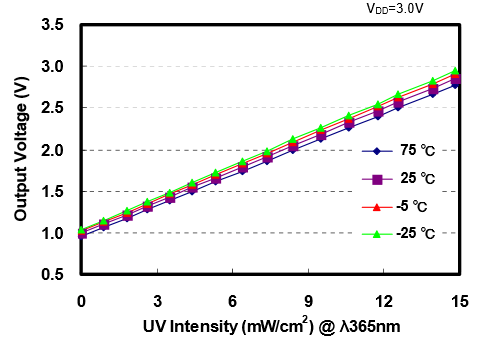
\includegraphics[scale=0.4]{2_Beschreibung_des_CANSAT/graph_photodiode_response.png}
	\caption{Spannungsausgabe vs. UV Intensität}
	\label{graph photodiode}
\end{figure}


\paragraph{Sharp Feinstaubsensor}
Der Sharp Feisensor arbeite, wie der ML8511, sehr simpel. Im inneren befindet sich eine Infarot Diode welche die Partikel anstrahlt, auf der anderen Seite befindet sich ein Fototransistor welcher dann feststellt wieviel von diesem Licht von Partikeln reflektiert wird, diese Veränderung ist messbar.

\begin{figure}[h]
	\centering
	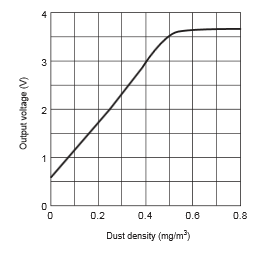
\includegraphics[scale=0.5]{2_Beschreibung_des_CANSAT/graph_photodiode_sharp.png}
	\caption{Spannungsausgabe vs. Staub}
	\label{graph photodiode}
\end{figure}

Um den Fototransistor nicht immer ganz zu bestrahlen, ist die Infarot Diode nicht die gesamte Zeit angeschaltet sonder nur einen Bruchteil einer Sekunde, die Messung muss inerhalb dieser Zeitspanne passieren.

\begin{figure}[h]
	\centering
	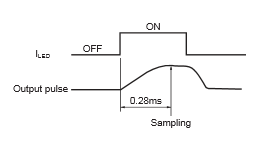
\includegraphics[scale=0.5]{2_Beschreibung_des_CANSAT/graph_output_sampling.png}
	\caption{Zeitspanne einer Messung}
	\label{sampling}
\end{figure}

\paragraph{APC220}
Der APC220, ist ein Transciever welcher entweder senden oder empfangen kann. Der BeagleBone Black schickt den formatierten JSON String per UART an den APC220, dieser schickt ihn über die vorher am Computer festgelegte Frequenz in den Raum weiter. Am Boden befindet sich ebenfalls ein APC220, welcher die Daten empfängt.

\paragraph{Ultimate GPS}
Der Ultimate GPS von Adafruit verbindet sich mit den allgemeinen GPS-Satelliten und sendet Serial seine Daten im NMEA Format aus, aus diesen können wir dann verschiedene Daten auslesen:

\begin{table}[H]
  \centering
    \begin{tabular}{rr}
    \toprule
    \textbf{Nummer} & \textbf{Daten} \\
    \midrule 
    1 & Breitengrad \\
    2 & Längengrad \\
    3 & Zeit \\
    4 & GPS-Qualität \\
    5 & Anzahl benutzter Satelliten \\
    6 & Höhe \\
    \bottomrule
    \end{tabular}
    \caption{Auslesebare Daten}
\end{table}

Außerdem können wir den Ultimate GPS über die serielle UART Schnittstelle konfigurieren um ihn zum Beispiel nur ein bestimmtes NMEA Format ausgeben zu lassen oder um die Bitrate der seriellen Übertragung zu ändern.

\paragraph{TMP006}
Der TMP006 ist ein Infarot Temparatur Sensor, welcher die Temperatur von einem Objekt misst ohne in direktem Kontakt zu stehen. Der Sensor misst die Temperatur eines Objektes anhand der ausgestrahlten Energy auf Wellenlänge von 4 micrometers bis zu 16 micrometers. Durch die veränderte Spannung am Sensor ist eine Messung der Temperatur möglich. Je größer das Objekt umso weiter entfernt muss es sich befinden um vom Sensor Field of View erfasst zu werden.

\begin{figure}[h]
	\centering
	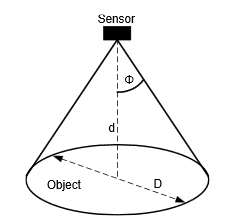
\includegraphics[scale=0.5]{2_Beschreibung_des_CANSAT/sensor_fov.png}
	\caption{Sensor Field of View}
	\label{sensor fov}
\end{figure}

Die Messung kann sehr ungenau werden da je nach Aussentemperatur und Temperatur der Sensorfläche selber Fehler beim Messen enstehen können.

\paragraph{BMP180}
Der BMP180 ist ein Drucksensor welcher mithilfe einer Membran den Druck misst und per On-Board Controller diesen direkt in die Höhe umrechnet. Der Sensor sendet die Daten dann per I²C-Bus an uns weiter.

\subsubsection{Energieverbrauch}
\begin{table}[H]
  \centering
    \begin{tabular}{rrrl}
    \toprule
    \textbf{Bauteil} & \textbf{Stromaufnahme} & \textbf{Spannung} & \textbf{Leistungsaufnahme} \\
    \midrule
    Beaglebone Black  & 500mA & 5V & 2500mW \\
    ML8511& <1mA & 3.3V & <3.3mW \\
    TMP006& <1mA& 3.3V& <3.3mW \\
    Sharp& 20mA & 3.3V& 66mW\\
    BMP180& <1mA& 3.3V& <3.3mW \\
    Ultimate GPS Modul& 25mA&3.3V& 82.5mW \\
    APC220& 35mA & 5V & 175mW\\

    \bottomrule
     & & &2833.4mW \\
    \bottomrule
    \end{tabular}%
    \caption{Energieverbrauch}
  \label{tab:budgetausgaben}%
\end{table}%
